\documentclass[tikz,border=2pt]{standalone}
\usepackage{amsmath,amssymb}
\usepackage{tikz}

\begin{document}
% The sample space S lists every possible outcome of the experiment: the six faces of a die,
% or the four results of tossing two coins.
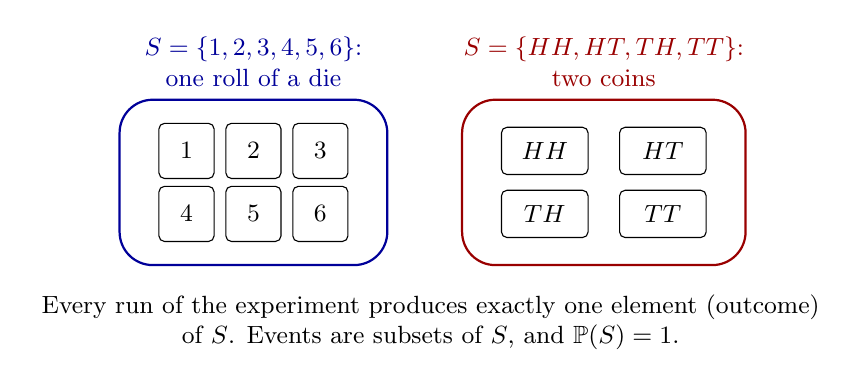
\begin{tikzpicture}[every node/.style={font=\small}]
	\draw[thick, blue!60!black, rounded corners=12pt] (-0.35,-0.3) rectangle (3.05,1.8);
	\node[blue!60!black, anchor=south, align=center] at (1.35,1.85) {$S=\{1,2,3,4,5,6\}$:\\ one roll of a die};
	\foreach \i in {1,...,6} {
		\pgfmathsetmacro{\x}{0.5+mod(\i-1,3)*0.85}
		\pgfmathsetmacro{\y}{\i<4 ? 1.15 : 0.35}
		\node[draw, fill=white, rounded corners=2pt, minimum size=7mm] at (\x,\y) {$\i$};
	}
	\draw[thick, red!60!black, rounded corners=12pt] (4.0,-0.3) rectangle (7.6,1.8);
	\node[red!60!black, anchor=south, align=center] at (5.8,1.85) {$S=\{HH,HT,TH,TT\}$:\\ two coins};
	\foreach \lab/\x/\y in {HH/5.05/1.15, HT/6.55/1.15, TH/5.05/0.35, TT/6.55/0.35} {\node[draw, fill=white, rounded corners=2pt, minimum width=1.1cm, minimum height=6mm] at (\x,\y) {$\lab$};}
	\node[anchor=north, align=flush center, text width=10cm] at (3.6,-0.55) {Every run of the experiment produces exactly one element (outcome) of $S$. Events are subsets of $S$, and $\mathbb{P}(S)=1$.};
\end{tikzpicture}
\end{document}
